\section{Installationsvorbereitungen}
\label{sec:installation}
In diesem Kapitel werden die Schritte erklärt, die durchgeführt werden müssen, bevor man die .apk-Datei erzeugen lassen kann.

\subsection{Erforderliche Schnittstellen}
Zunächst muss ein Backend System verfügbar sein. Dieses muss einige Schnittstellen bieten, die nachfolgend erläutert werden. Zusätzlich ist es erforderlich, dass alle Anfragen in JSON empfangen werden können und alle Antworten in JSON vorliegen.

\subsubsection{Registrationsschnittstelle}
\begin{figure}[h]
	\centering
	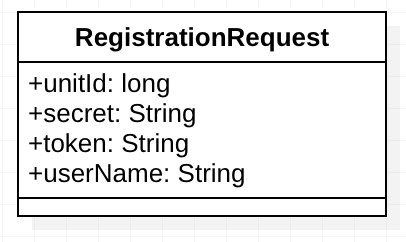
\includegraphics{include/img/registrationrequest}
	\caption{RegistrationRequest}
	\label{fig:registrationrequest}
\end{figure}

Die Registrationsschittstelle muss unter dem Endpunkt \textit{/registration} per POST-Methode erreichbar sein. Im RequestBody wird ein sog. \textit{RegistrationRequest} mitgeschickt, der in Abbildung~\ref{fig:registrationrequest} zu sehen ist. Die Daten um die Anfrage zu befüllen stammen aus dem QR-Code (UnitID, Secret) beziehungsweise aus der App des Benutzers (Token, Name).

\begin{figure}[h]
	\centering
	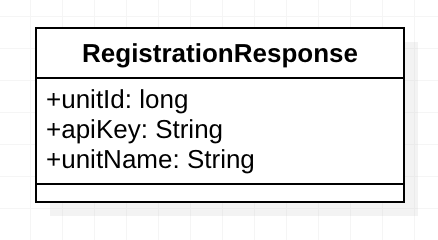
\includegraphics{include/img/registrationresponse}
	\caption{RegistrationResponse}
	\label{fig:registrationResponse}
\end{figure}
Als Ergebnis auf die Anfrage erwartet die App eine \textit{RegistrationResponse}, die in Abbildung~\ref{fig:registrationResponse} dargestellt ist. In diesem Objekt liegt ein generierter API Schlüssel, der quasi das Passwort des Benutzers darstellt um sich beispielsweise abzumelden.

\begin{figure}[h]
	\centering
	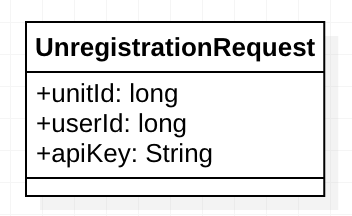
\includegraphics{include/img/unregistrationrequest}
	\caption{UnregistrationResponse}
	\label{fig:unregistrationResponse}
\end{figure}

Um diese Abmeldung zu realisieren muss die Schnittstelle eine weitere Funktionalität bieten. Diese erfolgt ebenfalls auf dem Endpunkt \textit{/registration}, nur ist dieses mal die DELETE Methode erforderlich. Zusätzlich wird wieder im RequestBody ein Objekt mitgeschickt, das wie in Abbildung~\ref{fig:unregistrationResponse} aussehen muss. Als Antwort wird ein Http-Status 204 (No-content) zurückgeliefert, wenn die Registration gelöscht wurde. Falls nicht, kann ein beliebiger anderer Status zurückgegeben werden. Um aber möglichst nahe an REST zu bleiben bieten sich insbesondere die Statuscodes der Bereiche 4xx (Client Fehler) und 5xx (Server Fehler) an.

\begin{figure}[h]
	\centering
	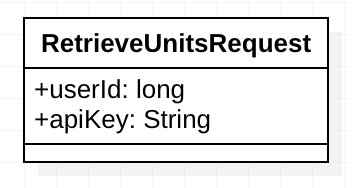
\includegraphics{include/img/retrieveunitsrequest}
	\caption{RetrieveUnitsRequest}
	\label{fig:retrieveUnitsRequest}
\end{figure}
Zuletzt muss diese Schnittstelle auch einen Endpunkt bieten um alle aktuell registrierten Einheiten eines Benutzers auszulesen. Diese muss \textit{/units} mit POST angeboten werden. Das ist zwar nicht absolut REST-konform, aber die GET-Methode bietet keine Möglichkeit einen RequestBody anzuhängen. Parameter, die direkt in der URL mitgegeben werden, können unter Umständen abgehört werden. Im Body liegt ein RetrieveUnitsRequest, der in Abbildung~\ref{fig:retrieveUnitsRequest} zu sehen ist.

\begin{figure*}
	\centering
	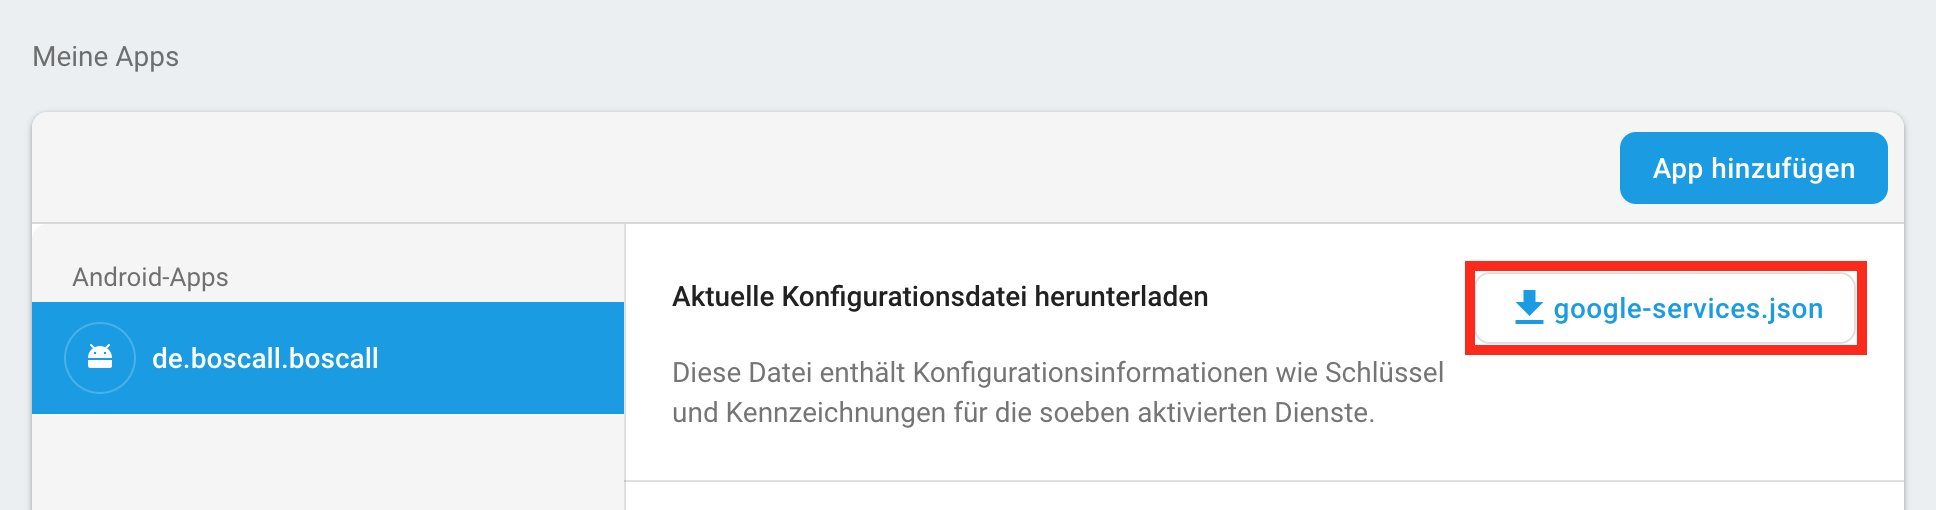
\includegraphics[width=\linewidth]{include/img/google-services-json}
	\caption{google-services.json Download}
	\label{fig:google-services-json-download}
\end{figure*}

\subsubsection{Tokenschnittstelle}
\begin{figure}[h]
	\centering
	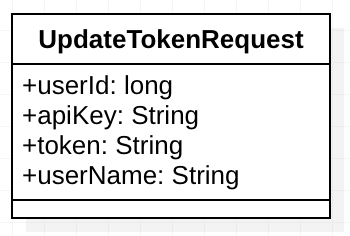
\includegraphics{include/img/updatetokenrequest}
	\caption{UpdateTokenRequest}
	\label{fig:updateTokenRequest}
\end{figure}
Die Tokenschnittstelle dient der App dazu, bei einer Änderung eines Tokens eines Benutzers diesen in der Datenbank des Backends zu aktualisieren. Da der Token die einzige Möglichkeit ist, das Endgerät mittels Push Nachrichten zu adressieren sind solche Anfragen enorm wichtig. Zusätzlich wird der Endpunkt genutzt um bei einer lokalen Änderung eines Benutzernamens diesen auch in der Datenbank des Backends zu aktualisieren. Der Endpunkt \textit{/updateToken} muss für die POST-Methode angeboten werden. Es wird hierbei ein UpdateTokenRequest, zu sehen in Abbildung~\ref{fig:updateTokenRequest}, mitgeschickt. Als positives Ergebnis wird der Statuscode 200 (OK) erwartet.

\subsubsection{Kalenderschnittstelle}
Die letzte erforderliche Schnittstelle ist die Kalenderschnittstelle, die bei Anfrage alle Termine eines Benutzers zurückliefert. Dieser Endpunkt ist unter \textit{/calendar} mittels GET erreichbar und es wurde sich deutlich mehr an die Vorgaben des REST Stils gehalten. Hier gilt es in Zukunft zu evaluieren, ob die Sicherheit des API Schlüssels in den Parametern der URL gewährleistet ist. Jedenfalls wird die UserId und der API Schlüssel als Parameter in der URL übertragen. Ein Beispiel mit der UserId 42 und dem API Schlüssel 1234567890: \textit{/calendar/userId=42\&apiKey=1234567890}.

\begin{figure}[h]
	\centering
	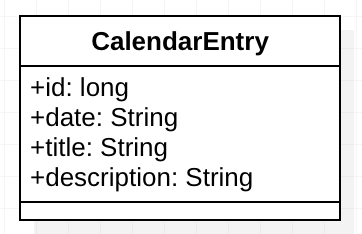
\includegraphics{include/img/calendarentry}
	\caption{CalendarEntry}
	\label{fig:calendarEntry}
\end{figure}
Als Antwort erwartet die App eine Liste (in JSON ein Array - \enquote{[ ]}) aus CalendarEntry-Objekten. Diese sind aufgebaut wie in Abbildung~\ref{fig:calendarEntry} dargestellt.

\subsection{Erforderliche Konfiguration der App}
Damit die App später auch das richtige Backend anspricht ist es erforderlich dessen Adresse anzupassen. Die Anpassung erfolgt in der Klasse\\ \textit{de.boscall.constants.ServiceConfiguration}. Die dortigen Anpassungen sind dann selbsterklärend.

Zuletzt muss dann in das \enquote{app}-Verzeichnis eine sog. \enquote{google-services.json}-Datei gelegt werden. Diese bekommt man in der Firebase Console. In den Einstellungen des Projekt befindet sich direkt auf der Startseite ein Button \enquote{google-servies.json}, mit dem man die Datei herunterladen kann. Der Button ist auch in Abbildung~\ref{fig:google-services-json-download} farblich hervorgehoben. In der Datei sind Daten hinterlegt um mit Firebase kommunizieren zu können. Insbesondere der API Schlüssel und die Projektkennung.